\documentclass[ignorenonframetext]{beamer}

\usepackage[english]{babel}
\usepackage{ucs}
\usepackage[utf8x]{inputenc}
\usepackage[T1]{fontenc}
\usepackage{hyperref}

\def\museincludegraphics{%
  \begingroup
  \catcode`\|=0
  \catcode`\\=12
  \catcode`\#=12
  \includegraphics[width=0.50\textwidth]
}

\title{Det (o)nödvändiga jaget}
\author{Henrik Frisk}
\date{December  4, 2012}

\begin{document}

\frame{\titlepage}

\begin{frame}[fragile]
\frametitle{(Re)thinking Improvisation}

VR-projekt som startade 2009 och avslutas i februari.
\vspace{0.5cm}
Mynnade ut i en stor konferens i November 2011: (Re)thinking Improvisation: International sessions in artistic research
\end{frame}

\begin{frame}
  \frametitle{Improvisation, Computers and Interaction}

  \begin{center}
    \includegraphics[width=.3\textwidth]{img/imp-comp-int.png}
    % 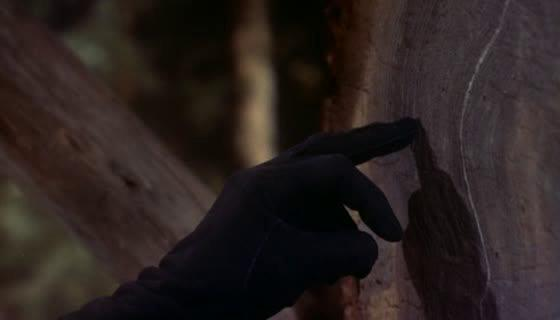
\includegraphics[width=.8\textwidth]{media/vertigo-finger.jpg}
  \end{center}
  \begin{center}
    \emph{Improvisation, Computers, and Interaction: Rethinking Human-Computer Interaction Through Music}
  \end{center}
  \uncover<2->{
    \begin{center}
      (\url{www.performingarts.lu.se})
    \end{center}
  }

\end{frame}

\begin{frame}
  \frametitle{Improvisation, motstånd och Interaktion}
  
Att förstå improvisation utifrån sig självt, utifrån dess egna förutsättningar och hur dessa interagerar med jaget såsom det manifesterar sig genom improvisation. Dessa tre, improvisation, teknik och jaget, är helt uppenbart inte jämförbara enheter och kan därför inte ses som poler, men deras banor korsas ofta, och när så sker uppstår friktion.

\vspace{0.5cm}

Teknikens substantiella skillnad (och fördel) framför instrumentets.

\end{frame}

\begin{frame}
  \frametitle{Motstånd}
  \begin{enumerate}
  \item<1> Idiomatiskt motstånd
  \item<2> Instrumentets motstånd
  \item<3> Psykologiskt motstånd
  \item<4> Kulturellt motstånd
  \item<5> \ldots
  \end{enumerate}
\end{frame}

\begin{frame}
  \frametitle{Improvisation som metod}
  
  \begin{itemize}[<+->]
  \item Vad kan jag kontrollera?
  \item Vad kan jag förstå?
  \item Vad kan jag förbereda och vad måste jag lämna utanför min kontroll?
  \end{itemize}

\end{frame}

\begin{frame}
  \frametitle{The six tones och mötet med den andre}
  Mötet med en främmande musikkultur ställer jaget och den andre samt begrepp som kulturellt motstånd i centrum.

  Tu Dai O\'{a}n: en studie i tvärkulturell interaktion i improvisation.
  
\end{frame}

\begin{frame}
  \frametitle{Angreppets förändringsprocess}
  
  Min relation till uppgiften förändrades olika till hur Stefans relation förändrades.

  \vspace{0.5cm}

  Mötet skapar individuella behov för förutsättningar.

\end{frame}

\begin{frame}
  \frametitle{Filosofiska betraktelser över jaget}
  \begin{itemize}[<+-]>
  \item Husserl
  \item Hegel 
  \item Sartre
  \item Habermas
  \item Levinas: face-à-face
  \item \ldots
  \end{itemize}
\end{frame}

\begin{frame}
  \frametitle{Avgränsningens estetik}
  
  Konstnärliga forskning har ett inbyggt problem i att det alltid finns en risk att arbetet blir dubbelt eller trippelt. Att krav ställs på t.ex. både konstnärlig och teoretisk skicklighet på ett sätt som skapar problem.
  
\end{frame}

\begin{frame}
  \frametitle{Att lyssna på den andre}
  \begin{itemize}[<+->]
  \item Centralt begrepp. Enligt Levinas kan relationen inte reduceras till identitet ($$ A \ne B $$) och inför samtidigt ett ansvar för den andre i jaget.
  \item Lyssnandet i musikalisk interaktion är centralt - resonansen (Nancy)
  \item Men vad är det man lyssnar när man lyssnar?
  \item Vad är det som ska påverkas och vad är det som ska förbli opåverkat?
  \item Vad är identitet och vad är interaktion?
  \end{itemize}
\end{frame}

  \begin{frame}
    \frametitle{Identitet}
    Att skapa en musikalisk identitet och ett personligt uttryck är viktigt, inte minst i jazzen.

    \begin{itemize}[<+->]
    \item Coleman Hawkins
    \item Betty Carter
    \item Charlie Parker
    \item Billie Holiday
    \item Carla Bley
    \item Albert Ayler
    \end{itemize}

    Deras identitet är deras `sound'. Originalitet är ett estetiskt värdeord.
  \end{frame}

  \begin{frame}
    \frametitle{Det rena uttrycket}
    
    Ornette Coleman: ``Kreativitet utan minne''

    Marcel Duchamp: Traditionens fängelse, ``I unlearned to draw. The point was to forget with my hand.''

    Denardo Coleman: Spelar utan att bry sig om politiken utan är helt enkelt fri.

  \end{frame}

  \begin{frame}
    \frametitle{I have nothing to say and I am saying it}
    
    När jaget befrias från sina intentioner.
    \vspace{0.5cm}

    Alltså, till skillnad från jazzens fokus på identitet och individuellt uttryck vill Cage uppleva världen och omgivningen så som den är, inte skapa en kopia av den.
    \vspace{0.5cm}

    Duchamp:

    the difference between the artistic intention and its realization goes unnoticed by the artist and it represents his (or her) inability ``to express fully his intention''. 

    ``the personal ’art coefficient’ is like an arithmetical relation between the unexpressed but intended and the unintentionally expressed.''
  \end{frame}

  \begin{frame}
    \frametitle{Thoureau}
    Det är först när man upphör att försöka förstå som man verkligen kan betrakta eller höra.
    \vspace{0.5cm}

    Bort från det personliga uttrycket och mot det föränderliga jaget som är mottagligt för yttre influenser. Det genomskinliga, närmast osynliga jaget ställs mot det jag som projicerar sig själv.

  \end{frame}

  \begin{frame}
    \frametitle{Bateson}

    [The] algorithms of the heart, or, as they say, of the unconscious, are, however, coded and organized in a manner totally different from the algorithms of language. And since a great deal of conscious thought is structured in terms of the logics of language, the algorithms of the unconscious are double inaccessible. It is not only that the conscious mind has poor access to this material, but also that when such access is achieved. e.g., in dreams, art, poetry, religion, intoxication, and the like, there is still a formidable problem of translation.

  \end{frame}

  \begin{frame}
    \frametitle{Avsaknad av relation}

    Avsaknaden av relation initialt i The Six Tones, i kombination med en analytisk (teoretisk) och reflekterande utgångspunkt, skapade kommunikationsproblemen som blev åtskilligt större än våraspråkliga problem.

  \end{frame}

  \begin{frame}
    \frametitle{Att lyssna eller att inte lyssna}
    
    Jaget är inte antingen det passiva lyssnande jaget eller det extroverta, projicerande men för att bibehålla kontakten med det inre är det nådvändigt att motstå vanan och nödvändigt att utveckla metoder för att försäkra sig om att det inte är vanan som styr utan lyssnandet. och därför måste jaget ibland ges upp för att det ska bli möjligt att återfinna det och den information och kunskap som det bär på.

  \end{frame}

  \begin{frame}
    \frametitle{Tack!}
    
  \end{frame}
\end{document}
